% v2-acmsmall-sample.tex, dated March 6 2012
% This is a sample file for ACM small trim journals
%
% Compilation using 'acmsmall.cls' - version 1.3 (March 2012), Aptara Inc.
% (c) 2010 Association for Computing Machinery (ACM)
%
% Questions/Suggestions/Feedback should be addressed to => "acmtexsupport@aptaracorp.com".
% Users can also go through the FAQs available on the journal's submission webpage.
%
% Steps to compile: latex, bibtex, latex latex
%
% For tracking purposes => this is v1.3 - March 2012

\documentclass[prodmode,acmtods]{acmsmall} % Aptara syntax

% Package to generate and customize Algorithm as per ACM style
\usepackage[ruled]{algorithm2e}
\renewcommand{\algorithmcfname}{ALGORITHM}
\SetAlFnt{\small}
\SetAlCapFnt{\small}
\SetAlCapNameFnt{\small}
\SetAlCapHSkip{0pt}
\IncMargin{-\parindent}

% Metadata Information
\acmVolume{1}
\acmNumber{1}
\acmArticle{1}
\acmYear{2015}
\acmMonth{4}

% Document starts
\begin{document}

% Page heads
\markboth{}{A General Framework for Geo-Social Query Processing
: An Experimental
Evaluation
}

% Title portion
\title{A General Framework for Geo-Social Query Processing
: An Experimental
Evaluation
}
\author{Spiros Desyllas
\affil{University of Piraeus}
}
% NOTE! Affiliations placed here should be for the institution where the
%       BULK of the research was done. If the author has gone to a new
%       institution, before publication, the (above) affiliation should NOT be changed.
%       The authors 'current' address may be given in the "Author's addresses:" block (below).
%       So for example, Mr. Abdelzaher, the bulk of the research was done at UIUC, and he is
%       currently affiliated with NASA.

\begin{abstract}
GeoSocial networks are systems consists of geo and social modules as presented in the work of Armenatzoglou et al.\cite{Armenatzoglou:geosn}. These modules work independently and collaborate in order to provide a framework of general Geo-Social query processing. In this paper we will try to evaluate this work by implementing a GeoSN network build upon NoSql Spatial capabilities. We examined different algorithm variations and measured the effectiveness of each in a thorough experiment. Finally we concluded by presenting which are the best algorithms for big amount of data.
\end{abstract}                                                                                     
          
\maketitle
% A category with the (minimum) three required fields
\section{Introduction}
A Geo-Social Network \cite{Armenatzoglou:geosn} is a system architecture that we can use in order to achieve a basic Geo-Social mechanism. According to this architecture a GeoSN network consists of : 

\begin{itemize}
  \item Social Module
  \item Geo Module
  \item Query Processing Module
\end{itemize}

The proposed architecture consists of three modules, depicted in
Figure 1: a social module (SM), a geographical module (GM), and
a query processing module (QM). The SM stores exclusively social
data (e.g., friendship relations), whereas the GM keeps only
geographical information (e.g., check-ins). The QM is responsible
for receiving GeoSN queries from users, executing them, and returning
the results. The users do not communicate directly with the
SM and GM. The SM, GM and QM can either be three separate
servers, three separate clouds, or a single system (server or cloud).
However, the tasks of the three modules are segregated.

\begin{figure}[h]
\centering
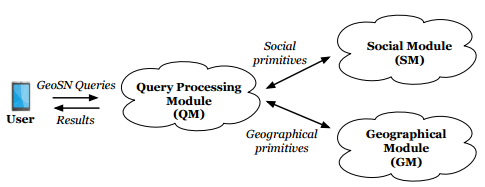
\includegraphics[width=0.7\linewidth]{./graphics/geoSNArchitecture}
\caption{Proposed GeoSN architecture}
\label{fig:geoSNArchitecture}
\end{figure}

A separation like this can provide numerous benefits such as administration by
different entities.The separation of QM enables third-party companies that do not own
any social or geographical data to implement GeoSN queries by
solely interacting with the APIs of SM and GM. In addition, separating the functionality of SM and GM renders
the management of social and geographical data more flexible, because
the frequent check-in updates do not burden the relatively
static social structures.

Finally, the segregation offers several other benefits. First of all the studied
architecture can readily integrate modifications (e.g., a new, more
efficient structure) in the implementation of SM without modifying
GM, and vice versa. Second, novel GeoSN query types and
algorithms can be devised, either by using a different combination
of existing primitives or by implementing new ones, without the
need of altering the SM and GM infrastructures. Last, social (geographical)
data can be used independently for pure social (resp.
geographical) queries, potentially through the same primitive operations
utilized by GeoSN queries. As a result, a “traditional” social
network can adopt this architecture without extra effort.

\section{Algorithms and variations}
The following algorithms are implemented in this paper in order to achieve complex queries like RangeFriends and NearestFriends

\subsection{Range Friends Algorithms}
Problem formulation. Simply stated, RF returns the friends of
user u that are within distance r to a location q. More formally:
PROBLEM 1. Given a user u, a 2D point q and a positive real
number r, a Range Friends (RF) query RF(u, q, r) returns a set
R defined as follows:
\newline
\newline
$  R = {ui | AreFriends(u, ui) ∧ ||q, ui|| ≤ r} $
\newline
\newline
Similar to RangeUsers and NearestUsers, the result contains
also the users’ locations. For example, RF(u4, q, 8) = {u2} and
RF(u5, q, 10) = {u1, u3}, where u1, u2, u3 carry both their ID
and location. This may be particularly useful for other GeoSN
queries that use RF as a subroutine, while it comes with a free
asymptotic cost (since the locations must be retrieved to answer the
query anyway, and do not add to the space complexity of the result).
We next describe three solutions for the RF query, whose pseudocode
is given in Figure 2.

\begin{figure}[h]
\centering
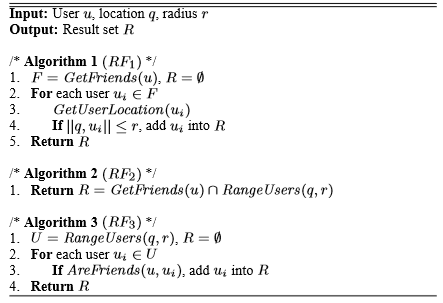
\includegraphics[width=0.7\linewidth]{./graphics/RF_algorithm}
\caption{Pseudocode of RF algorithms}
\label{fig:RF_algorithm}
\end{figure}


\textbf{Algorithm 1 (RF1)}
\newline
This variant first extracts the set F of u's
friends invoking primitive $GetFriends(u)$ in Line 1. Subsequently
(Lines 2-4), for every ui ∈ F, it retrieves its location via primitive
$GetUserLocation(ui)$, and inserts ui in result set R if the distance
between ui and q is smaller than or equal to r. For example,
$RF1(u4, q, 8)$ first computes $F = {u2, u3, u6}$ and retrieves the
user locations. Then, it adds only u2 to R, since $||q, u2|| = 6.4 ≤ 8
(||q, u3|| = 10 > 8, and ||q, u6|| = 12.2 > 8)$.

\textbf{Algorithm 2 (RF2)}
\newline
This algorithm gets the friends of u through
$GetFriends(u)$, and executes $RangeUsers(q, r)$ to get the users
that are within distance r to q. Finally, it performs an intersection
between these two sets, which yields the result R. For instance,
$RF2(u4, q, 8)$ performs $GetFriends(u4) ∩ RangeUsers(q, 8) =
{u2, u3, u6} ∩ {u1, u2} = {u2}$.

\textbf{Algorithm 3 (RF3)}
\newline
RF3 calculates $U = RangeUsers(q, r)$, and
then inserts ui into R if $AreFriends(u, ui) = true.$ In our
running example, $RF3(u4, q, 8)$ first executes $RangeUsers(q, 8)
= {u1, u2}$, and then calculates $AreFriends(u4, u1) = false$ and
$AreFriends(u4, u2) = true$. Consequently, the algorithm returns
$R = {u2}$ as the result.


The above algorithms have important differences. For instance,
RF2 and RF3 necessitate a spatial index for efficient range query
processing. RF3 could also benefit from an adjacency matrix implementation
(because it invokes AreFriends numerous times). In
addition, as we demonstrate in our experiments, the machine architecture
(centralized or distributed) has a significant impact on their
relative performance. Finally, the data and query parameters are
also vital in determining the best algorithm, e.g., if there are few
users within a range, RF2 and RF3 are preferable to RF1, while
RF1 is better for sparse social networks of users in the same geographic
area.

\subsection{Nearest Friends Algorithms}

Problem formulation. NF returns the k friends of user u that are
closest to location q in ascending distance. Formally:

\begin{figure}[h]
\centering
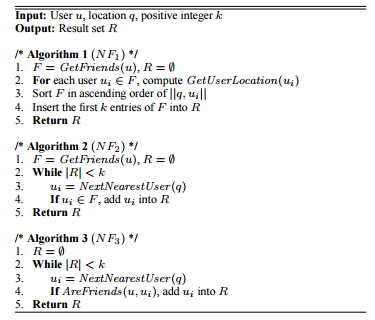
\includegraphics[width=0.7\linewidth]{./graphics/NF_algorithm}
\caption{Pseudocode of NF algorithms}
\label{fig:NF_algorithm}
\end{figure}

PROBLEM 2. Given a user u, a 2D point q and a positive integer
k, a Nearest Friends (NF) query NF(u, q, k) returns a list

For example, NF(u2, q, 2) = (u4, u6). Similar to the case of
RF, the result incorporates the user locations. Figure 3 includes the
pseudocode of three solution variants for NF, explained next:

\textbf{Algorithm 1 (NF1)}
NF1 first calculates F = GetFriends(u),
and gets the location of every ui ∈ F via GetUserLocation(ui).
Subsequently, it sorts F in ascending distance of each user therein
to q, and inserts the first k entries of F into R. In our example,
NF1(u2, q, 2) retrieves F = GetFriends(u2) = {u4, u6, u9},
extracts the user locations via three calls to GetUserLocation,
sorts F in ascending distance of each ui ∈ F to q producing ordered
list (u4, u6, u9). It finally returns the first 2 users in the list,
i.e., R = (u4, u6).

\textbf{Algorithm 2 (NF2)}
 NF2 first extracts the friends F of u through
GetFriends(u). It then iteratively retrieves the next nearest user ui
to q by calling NextNearestUser . If ui is in F, it is added to R.
When the size of R becomes equal to k, we are certain that we have
evaluated the correct result. In Figure 2, NF2(u2, q, 2) evaluates
F = GetFriends(u2) = {u4, u6, u9}. Then, it gets u1 as the
result of the first call to NextNearestUser (q). Since u1 6∈ F, it is
not added to R. Subsequently, it proceeds with retrieving users u2-
u6 through 5 calls to NextNearestUser (q), and adds only u4 ∈ F
and u6 ∈ F to R. At this point |R| becomes 2 and, thus, the
method returns R to the user and terminates.

\textbf{Algorithm 3 (NF3)}
NF3 is similar to NF2, but instead of invoking
GetFriends, it utilizes AreFriends for checking the friendship
between a user retrieved by NextNearestUser and u. In our running
example, NF3(u2, q, 2) iteratively computes users u1-u6 via
six calls to NextNearestUser , and performs an AreFriends primitive
for each of them. During this process, it adds u4, u6 to R
(since only those are friends with u2), and concludes $(|R| = 2)$.
Similar to the RF algorithms, the relative performance of the
NF solutions depends on the implementation, existing indexes, machine
architecture, data distribution, and query parameters

\section{Modules Implementation}
After examining the algorithm variations for these two type of queries (RF and NF) we proceed to the actual implementation of the modules.
For the implementation we used Ruby\cite{ruby} programming language for coding the api of the modules and the middleware of the database and MongoDB\cite{mongod} in order to store and index data.
We used MongoDB indexes in order to store social and geo data. For the social module we used MongoDB's single field to index the UserId and for the geo module we used GEO2D (2d Sphere) to index user location. We used GeoJSON\cite{geoJSON} to store user location as it is supported by MongoDB geospatial indexes. With the use of GEO2D index the Geo Module can perform the following basic geospatial queries as presented by Theodoridis et al. \cite{Corral:ClosestPair}

\begin{itemize}
  \item Point Location Query
  \item Range Query
  \item Join Query
  \item Nearest Neighbor Query
\end{itemize}


\subsection{Social Module}
The social module consists of a ruby class file which provides the following methods:
$getFriends(userid)$ and $areFriends(userid_1, userid_2)$. These two methods implement the primitive queries and mechanics for the social module. 
The $getFriends(userid)$ takes a userId as input and returns all the friends of the given user id in the form of a JSON \cite{json} array.
The $areFriends(userid_1, userid_2)$ method takes the ids of two users as input and returns
$True$ if the users are friends and $False$ if not

\subsection{Geo Module}
The geo module consists of a ruby class file which provides the following methods:
$nearestUsers(q, k)$, $getUserLocation(u)$ and $rangeUsers(q, r)$. These methods implement the primitive queries and mechanics for the geo module.
The nearestUsers method takes a query point q and an integer k as input and returns the k users nearest to q in ascending distance, along with their locations in a form of a JSON\cite{json} array.
The getUserLocation takes user id as an input and returns the user's location in the form a pair coordinate (latitude and longitude).
Finally rangeUsers takes a query point q and distance in meters r as input and returns the users within distance r from q, along with their locations, again in a form of JSON\cite{json} array.


\subsection{Query Processing Module}
The query processing module is a ruby class file which actually uses the above implemented modules in order to achieve more complex queries based on the primitive ones of the previous mentioned modules.
This module initially makes a connection to the social and geo module in order to be able to use their primitive mechanics. We stored geo and social data in MongoDB as already mentioned so this module uses Mongod Ruby driver in order to connect to MongoDB. Some portions of the driver are implemented in c++ for performance reasons. The methods implemented in this module are : rangeFriends and nearestFriends. We developed 3 different variations for each method based on the algorithms that we presented in the section above.
Method rangeFriends takes a user u , a 2D point q and a distance in meters r as input and returns all friends within the given range as a JSON array.
Method nearestFriends takes User u and a positive integer k as input and returns a JSON array consisting of friend's Id and friend's distance from q in ascending order.



\section{Evaluation and Running examples}
In order to initially provide synthetic data sets to modules we implemented a seed ruby program that randomly created users and geo locations based on random latitude and longitude. Each user has the two previous and two next created as friends. We then run a start up script in order to perform some queries to MongoDB and warm up caches. The first test run included 100 users and the second run test included 10000 users. We wanted to test algorithm variations with a small and a big data set to test if their performance was affected by the size of datasets. All the tests was run using an AMD A6 Dual Core Cpu clocked at 4.1Ghz and 4GB Ram. The datasets were stored in a regular HDD drive and MongoDB was set up in a Linux Ubuntu desktop distribution.

\section{Small DataSet measurements}
In the following tables we can see the test results for the small dataset of the 100 users
for the RangeFriends and Nearest Friends query processing
\newline

\textbf{Range Friends (RF) - 100 Records}
\begin{tabular}{|c|c|}
\hline \rule[-2ex]{0pt}{5.5ex} Aglorithm Variation & Execution Time (ms) \\ 
\hline \rule[-2ex]{0pt}{5.5ex} A & 2.33 \\ 
\hline \rule[-2ex]{0pt}{5.5ex} B & 9.64 \\ 
\hline \rule[-2ex]{0pt}{5.5ex} C & 52.42 \\ 
\hline 
\end{tabular} 

\begin{figure}[h]
\centering
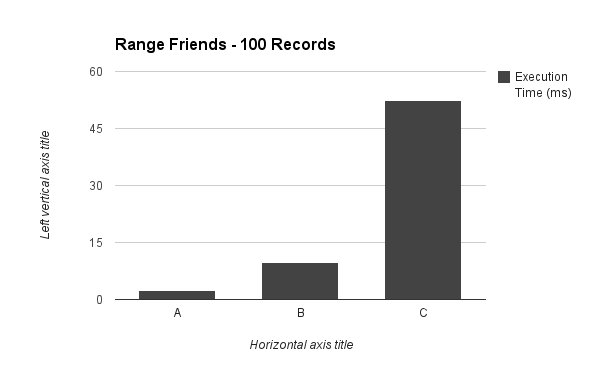
\includegraphics[width=0.7\linewidth]{./graphics/rf_100}
\caption{Range Friends (RF) - 100 Records}
\label{fig:nf_100}
\end{figure}

\clearpage{}
\textbf{Nearest Friends (NF) - 100 Records}
\begin{tabular}{|c|c|}
\hline \rule[-2ex]{0pt}{5.5ex} Aglorithm Variation & Execution Time (ms) \\ 
\hline \rule[-2ex]{0pt}{5.5ex} A & 1.34 \\ 
\hline \rule[-2ex]{0pt}{5.5ex} B & 3.73 \\ 
\hline \rule[-2ex]{0pt}{5.5ex} C & 47.11 \\ 
\hline 
\end{tabular} 

\begin{figure}[!h]
\centering
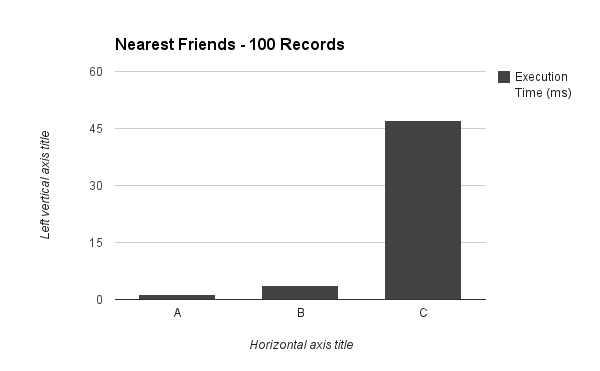
\includegraphics[width=0.7\linewidth]{./graphics/nf_100}
\caption{Nearest Friends (NF) - 100 Records}
\label{fig:nf_100}
\end{figure}

\section{Big DataSet measurements}
In the following tables we can see the test results for the big dataset of the 10000 users
for the RangeFriends and Nearest Friends query processing
\newline

\textbf{Range Friends (RF) - 10000 Records}
\begin{tabular}{|c|c|}
\hline \rule[-2ex]{0pt}{5.5ex} Aglorithm Variation & Execution Time (ms) \\ 
\hline \rule[-2ex]{0pt}{5.5ex} A & 8.37 \\ 
\hline \rule[-2ex]{0pt}{5.5ex} B & 298.43 \\ 
\hline \rule[-2ex]{0pt}{5.5ex} C & 4529.02 \\ 
\hline 
\end{tabular} 

\begin{figure}[h]
\centering
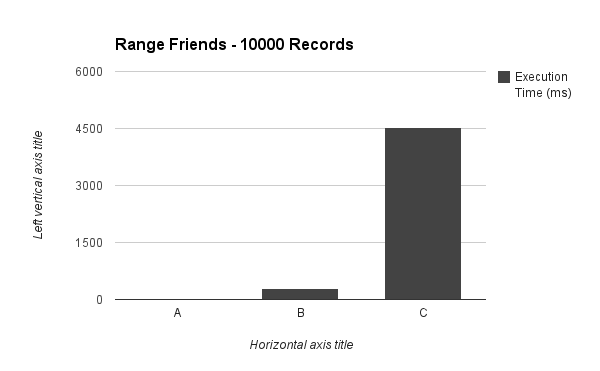
\includegraphics[width=0.7\linewidth]{./graphics/rf_10000}
\caption{Range Friends (RF) - 10000 Records}
\label{fig:nf_100}
\end{figure}


\textbf{Nearest Friends (NF) - 10000 Records}
\begin{tabular}{|c|c|}
\hline \rule[-2ex]{0pt}{5.5ex} Aglorithm Variation & Execution Time (ms) \\ 
\hline \rule[-2ex]{0pt}{5.5ex} A & 8.2 \\ 
\hline \rule[-2ex]{0pt}{5.5ex} B & 389.62 \\ 
\hline \rule[-2ex]{0pt}{5.5ex} C & 4856.17 \\ 
\hline 
\end{tabular} 

\begin{figure}[h]
\centering
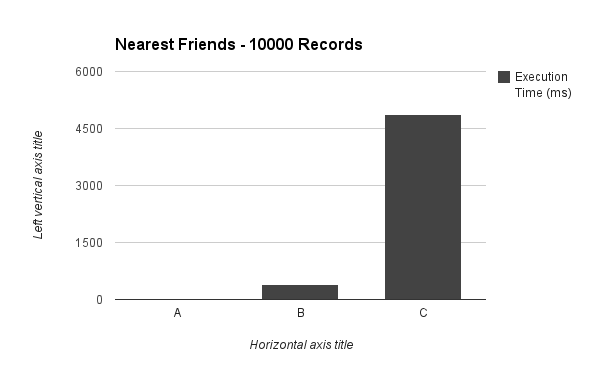
\includegraphics[width=0.7\linewidth]{./graphics/nf_10000}
\caption{Nearest Friends (NF) - 10000 Records}
\label{fig:nf_100}
\end{figure}


\clearpage{}
\section{Conclusions}
In this paper, we examined and experimented with an implementation of a Geo-Social network 
query processing system based on MongoDB geospatial indexes and programmed with Ruby. 
We evaluated 3 algorithm variations for each GeoSN query based on primitives queries implemented by primitive modules and evaluated each algorithm
implementation by measuring its process time against small and big amount of data. The queries that we experimented on were RangeFriends (RF) and NearestFriends (NF),
but a similar work needs to be done for GeoSN query NearestStarGroup (NSG). We used NoSql spatial capabilities for performance reasons but this experiment could be run on a 
classic relational DBMS as well, such us PostgreSQL. As a future work, further experiments can be done by testing bigger datasets with more complex queries.
%\end{document}  % This is where a 'short' article might terminate


% Bibliography
\bibliographystyle{abbrv}
%\bibliography{acmsmall-sample-bibfile}
\bibliography{spatialBibliography}
                             % Sample .bib file with references that match those in
                             % the 'Specifications Document (V1.5)' as well containing
                             % 'legacy' bibs and bibs with 'alternate codings'.
                             % Gerry Murray - March 2012



\end{document}
% End of v2-acmsmall-sample.tex (March 2012) - Gerry Murray, ACM


